\chapter{Solution Design}
\label{ch:design}

% ---------------------------------------------------------------------------
\section{Architectural Drivers and Overview}
\label{sec:arch-overview}
\label{sec:patterns}

Three requirements shape every structural decision in InfraArchAgent. FR-G-01
demands parallel execution of competing generator variants, which rules out a
simple sequential pipeline and forces an async orchestration model. FR-S-03
demands an iterative scan-remediate-rescan loop whose iteration count is
configurable at runtime, which rules out a fixed processing graph and forces
the SecurityAgent to own its own loop state. And NFR-03 demands that adding
a new LLM provider requires no changes to agent logic, which rules out
provider-specific code inside any agent and forces a provider abstraction layer
that sits between the agents and the network.

The architecture that satisfies all three is a four-layer system: a React
frontend, a FastAPI backend, an agent orchestration layer running on Python
asyncio, and a PostgreSQL data layer. Figure~\ref{fig:architecture} shows the
full system with its external dependencies.

\begin{figure}[h]
  \centering
  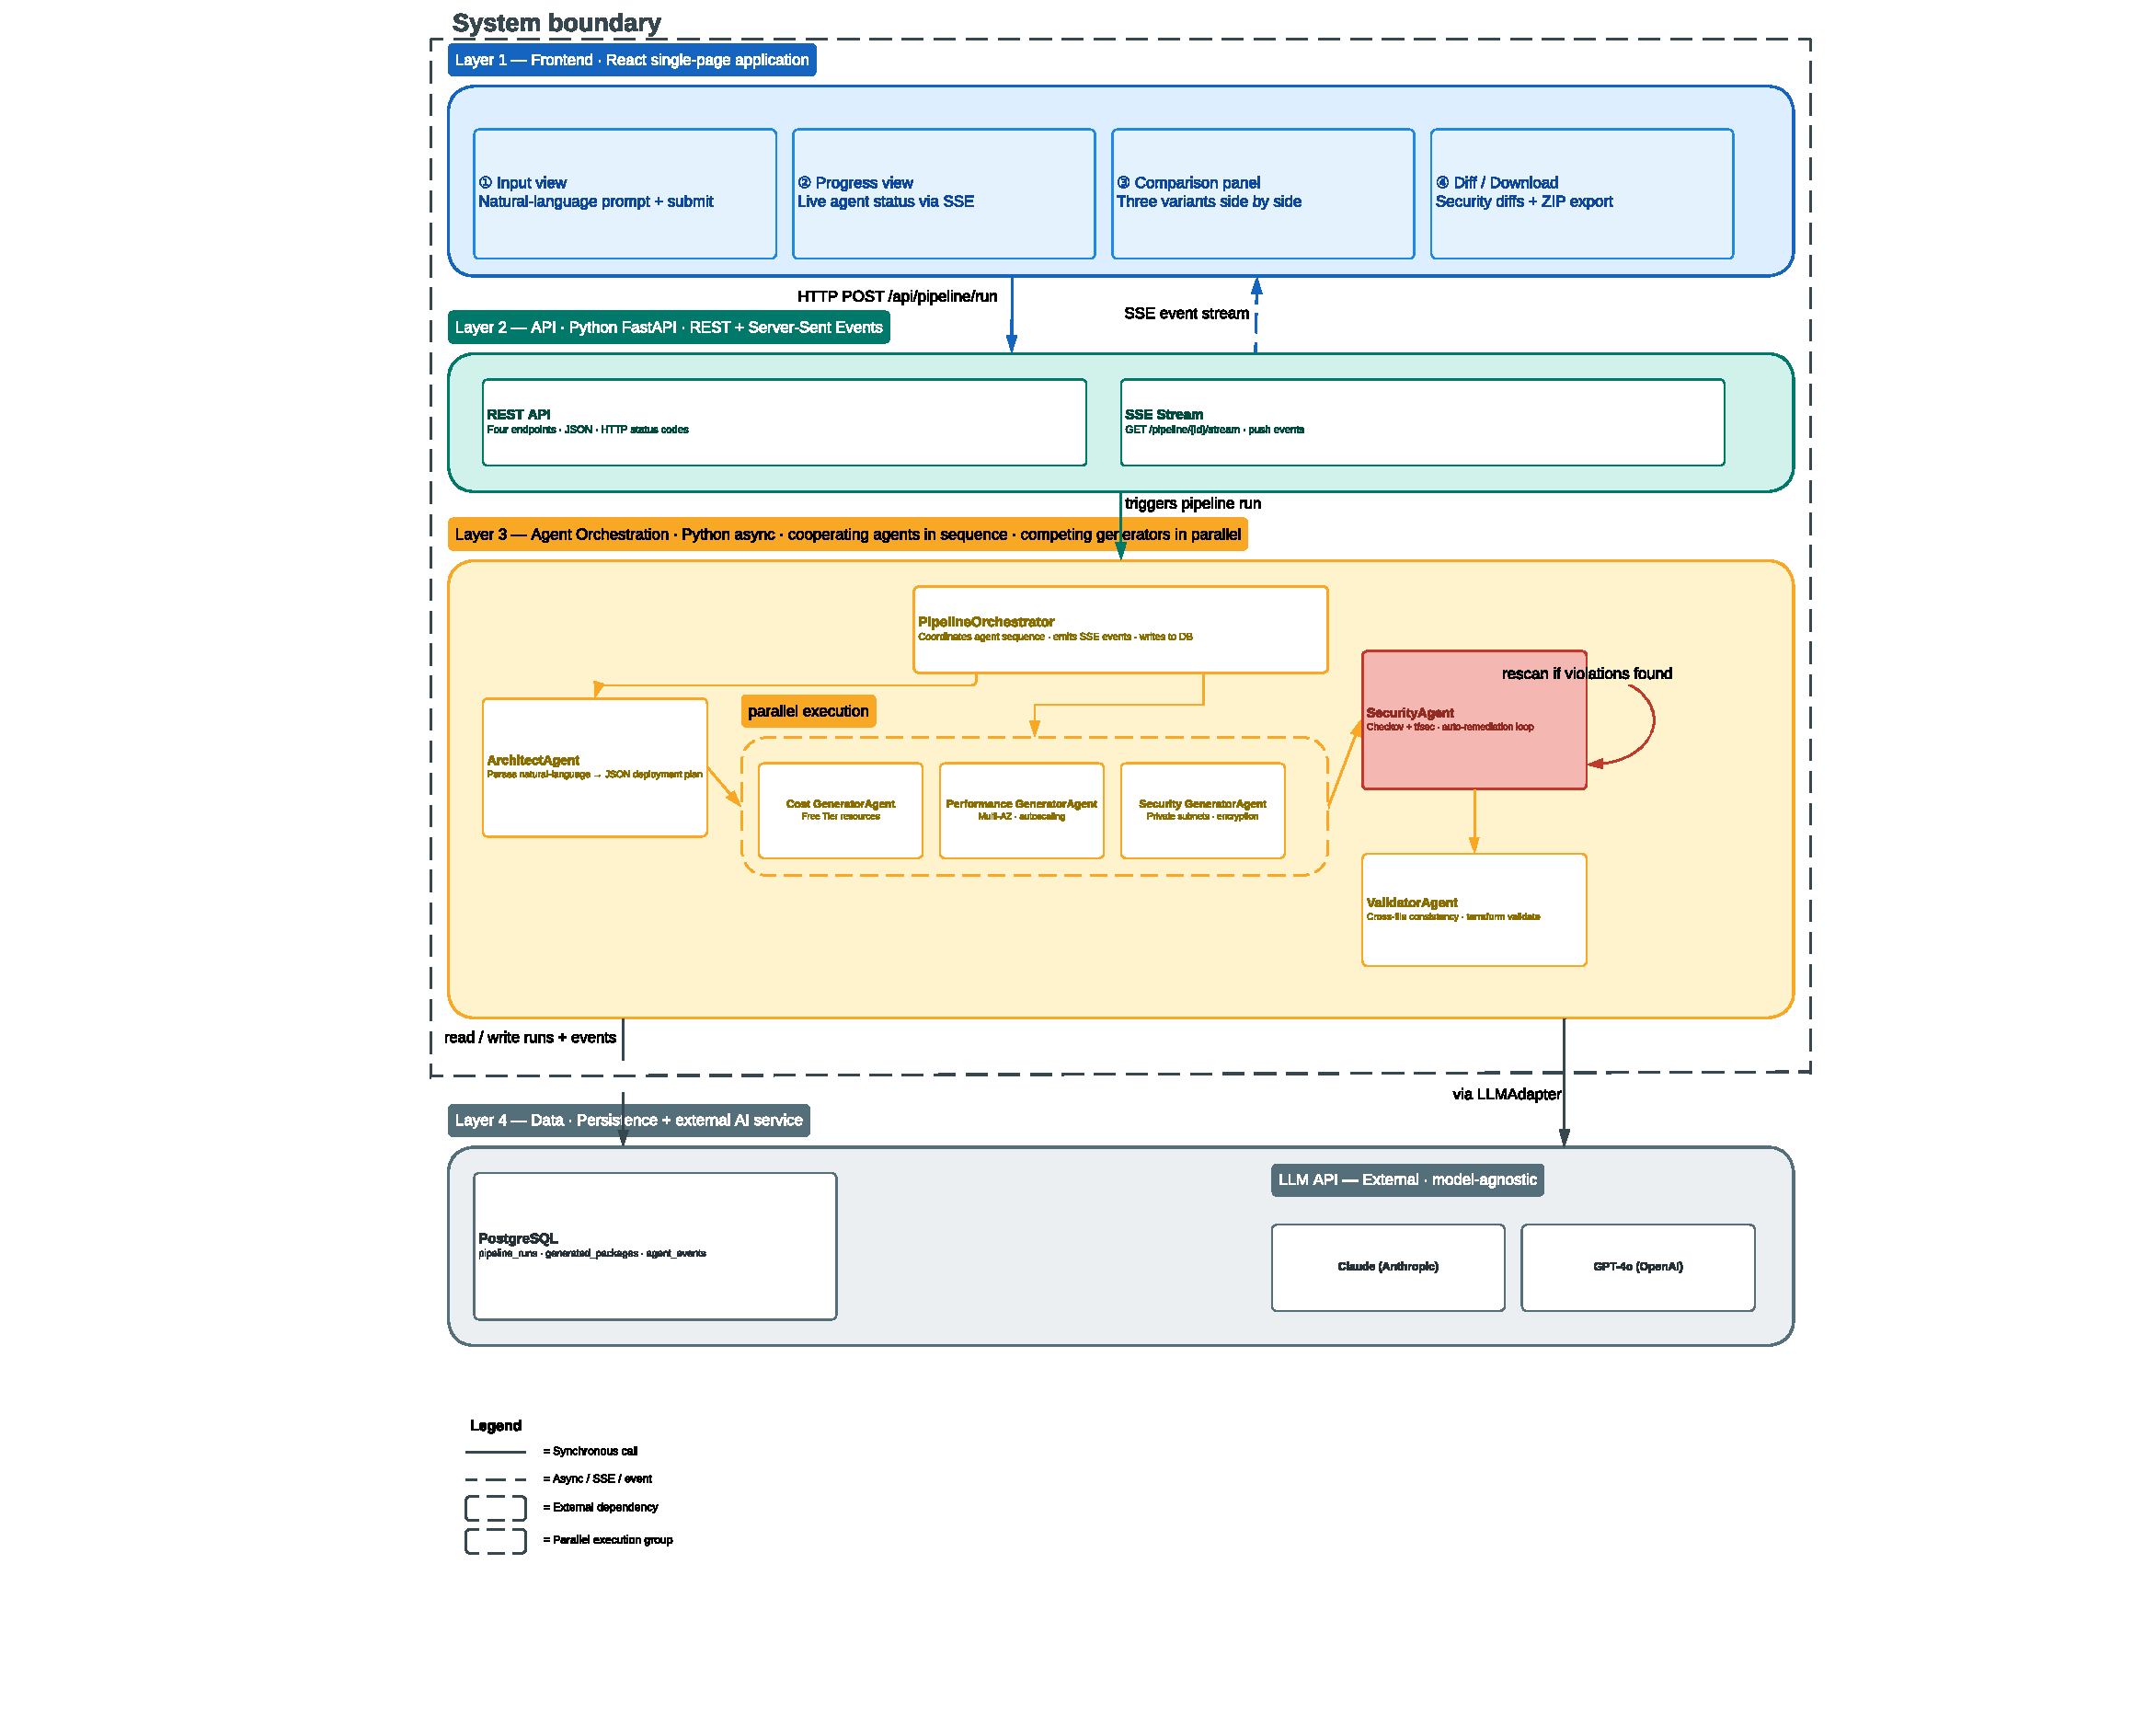
\includegraphics[width=\textwidth]{images/system_architecture.pdf}
  \caption{InfraArchAgent system architecture. Solid arrows are synchronous
    calls; dashed arrows are async or SSE events. The LLM API box has a dashed
    border because it is an external dependency outside the system boundary.}
  \label{fig:architecture}
\end{figure}

Each layer has one job. The frontend handles display and user interaction;
it contains no business logic. The API layer exposes four REST endpoints and
one SSE stream; it contains no agent logic. The orchestration layer runs the
pipeline; it contains no persistence logic beyond writing events to the queue.
The data layer stores everything; it contains no application logic. The
layering is strict: each layer talks only to the one directly below it, which
means the frontend can't reach the database and the agents can't reach the
browser.

The LLM API sits outside the boundary entirely. Agents reach it through the
LLMAdapter class, which wraps both the Anthropic Messages API and the OpenAI
chat completions API behind two methods. Swapping providers is a single
environment variable change; the agents don't know and don't need to.

% ---------------------------------------------------------------------------
\section{Business Rules and Domain Model}
\label{sec:domain}
\label{sec:class-design}

The pipeline has four invariants that hold across every run regardless of
input or configuration.

First, the ArchitectAgent's deployment plan is the sole input to the
GeneratorAgents. No generator reads the original natural-language string
directly (FR-A-05). This matters because the plan is structured and
unambiguous; the raw input is neither. Generators that re-interpret the
original string would produce inconsistent outputs across the three variants.

Second, a GeneratorAgent's package must contain every file type named in the
plan before it proceeds to the SecurityAgent (FR-G-02). A partial package
that passes security scanning would produce a downloadable ZIP that fails to
deploy.

Third, the remediation loop runs per-package, not per-pipeline. Each of the
three packages gets its own independent scan-fix-rescan cycle; a violation in
the cost variant doesn't affect the security variant's loop. This means the
three packages finish at different times and the SecurityAgent's overall
completion waits for all of them.

Fourth, pipeline failures are non-fatal below the ArchitectAgent level.
If one generator times out, the pipeline transitions to
\texttt{partial\_success} with the remaining packages (FR-P-03, FR-G-06).
If the ArchitectAgent fails, the pipeline halts entirely because there's no
plan for any generator to consume.

Fifth, no package reaches the engineer without a definitive readiness label.
A package that clears the remediation loop with zero violations and then
passes validation is marked \texttt{production\_ready} automatically; nobody
has to sign off on a clean result. A package that exhausts the iteration
limit with violations still outstanding stops there and waits (FR-S-07), and
so does a package that fails validation or whose ValidatorAgent crashes
before producing a report (FR-V-05). The SecurityAgent doesn't
guess, and it doesn't quietly hand over a half-fixed package labelled the
same as a fully-resolved one. That distinction is the whole point of the
\texttt{pending\_review} state: the engineer looks at what's left, and
either approves it as-is, sends it back with feedback for another pass, or
rejects it outright (FR-S-08 through FR-S-10). Whatever they choose, the
package ends up \texttt{production\_ready} or \texttt{not\_production\_ready}
--- never stuck in between, and never downloaded without the engineer
knowing which one it is.

Figure~\ref{fig:runstates} and Figure~\ref{fig:packagestates} show these
rules as UML state machines, one for the pipeline run as a whole and one
for each individual package moving through it.

\begin{figure}[h]
  \centering
  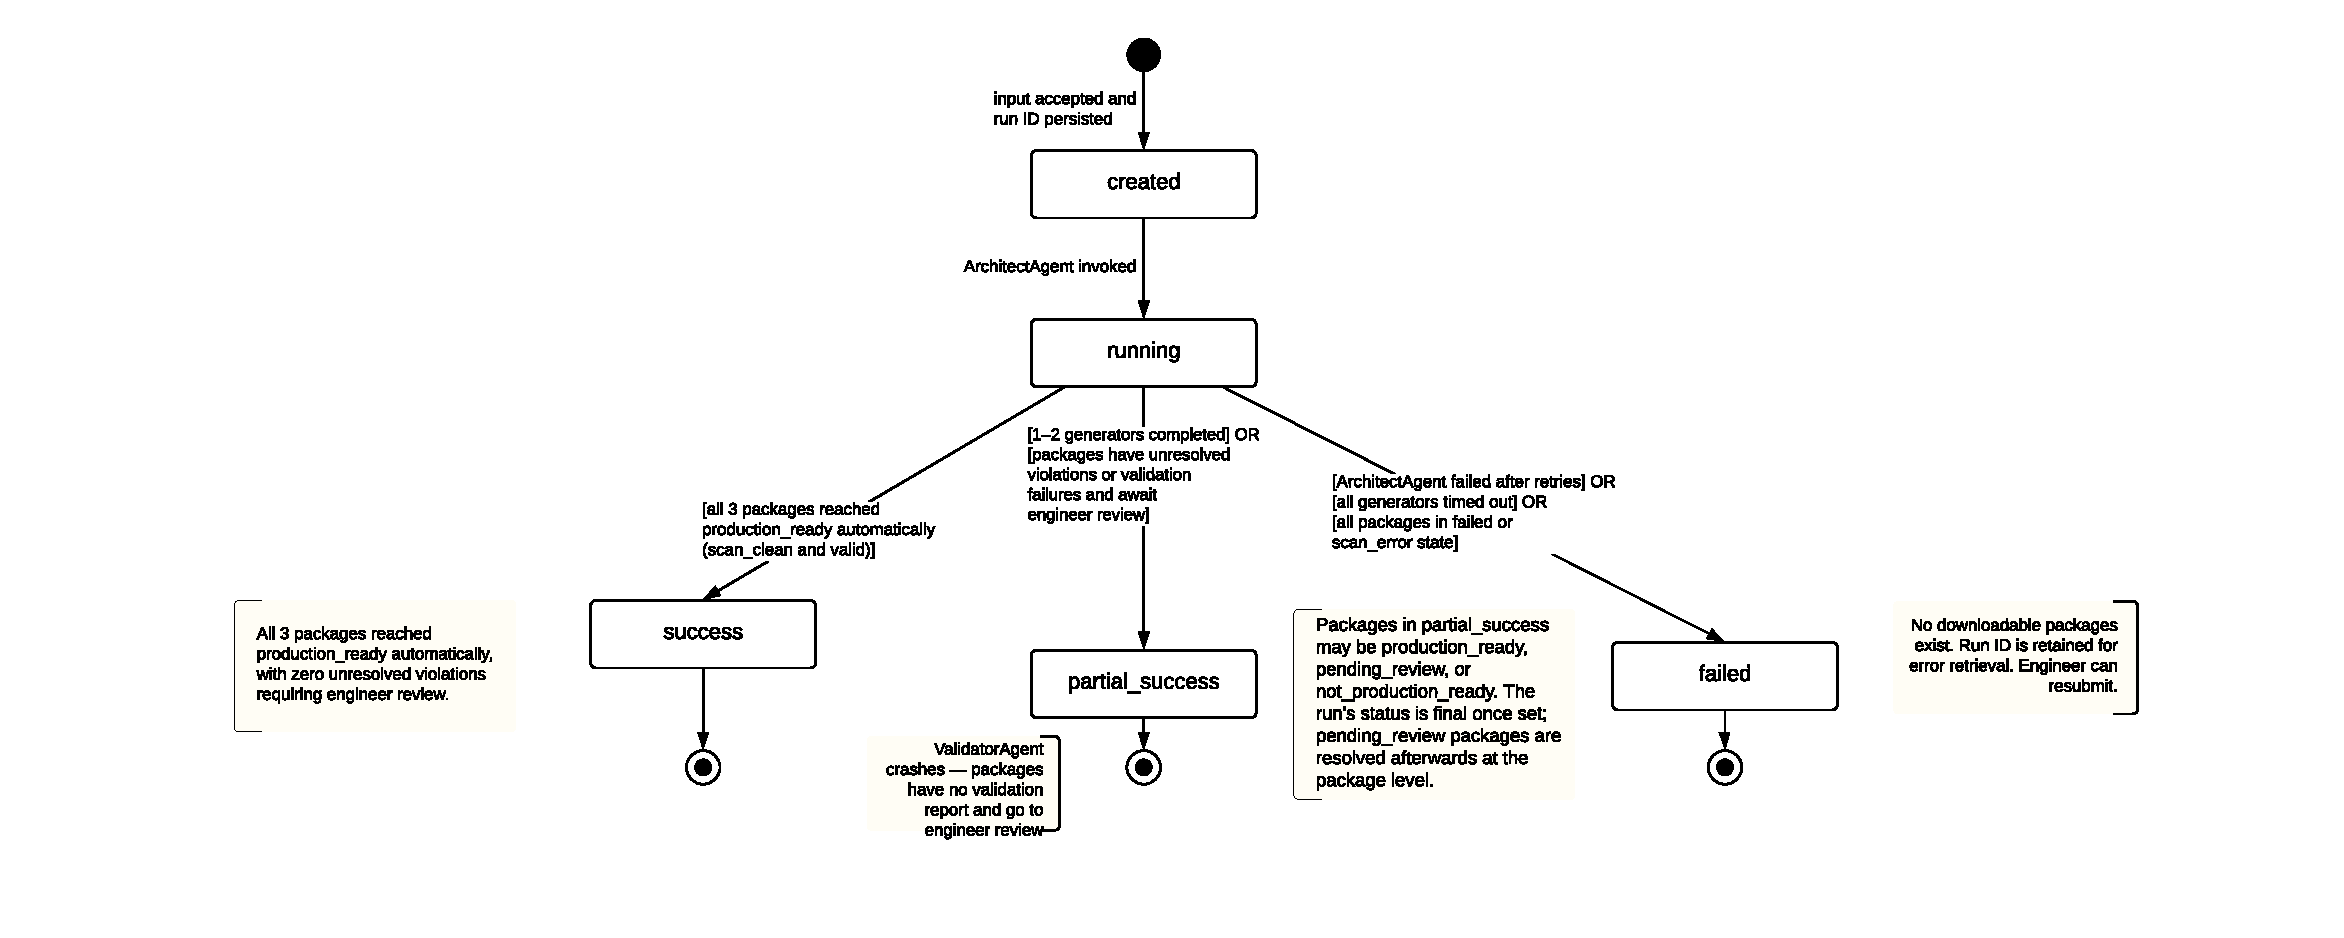
\includegraphics[width=\textwidth]{images/run_states.pdf}
  \caption{Run-level state machine. A run reaches \texttt{success} only
    when every package clears remediation and validation automatically;
    anything short
    of that lands in \texttt{partial\_success}, which may still contain
    packages awaiting engineer review. \texttt{failed} covers ArchitectAgent
    failure, total generator timeout, and the case where every package
    comes back with a scanner error. Drawn with AI-assisted prompting;
    reviewed and corrected by the author.}
  \label{fig:runstates}
\end{figure}

\begin{figure}[h]
  \centering
  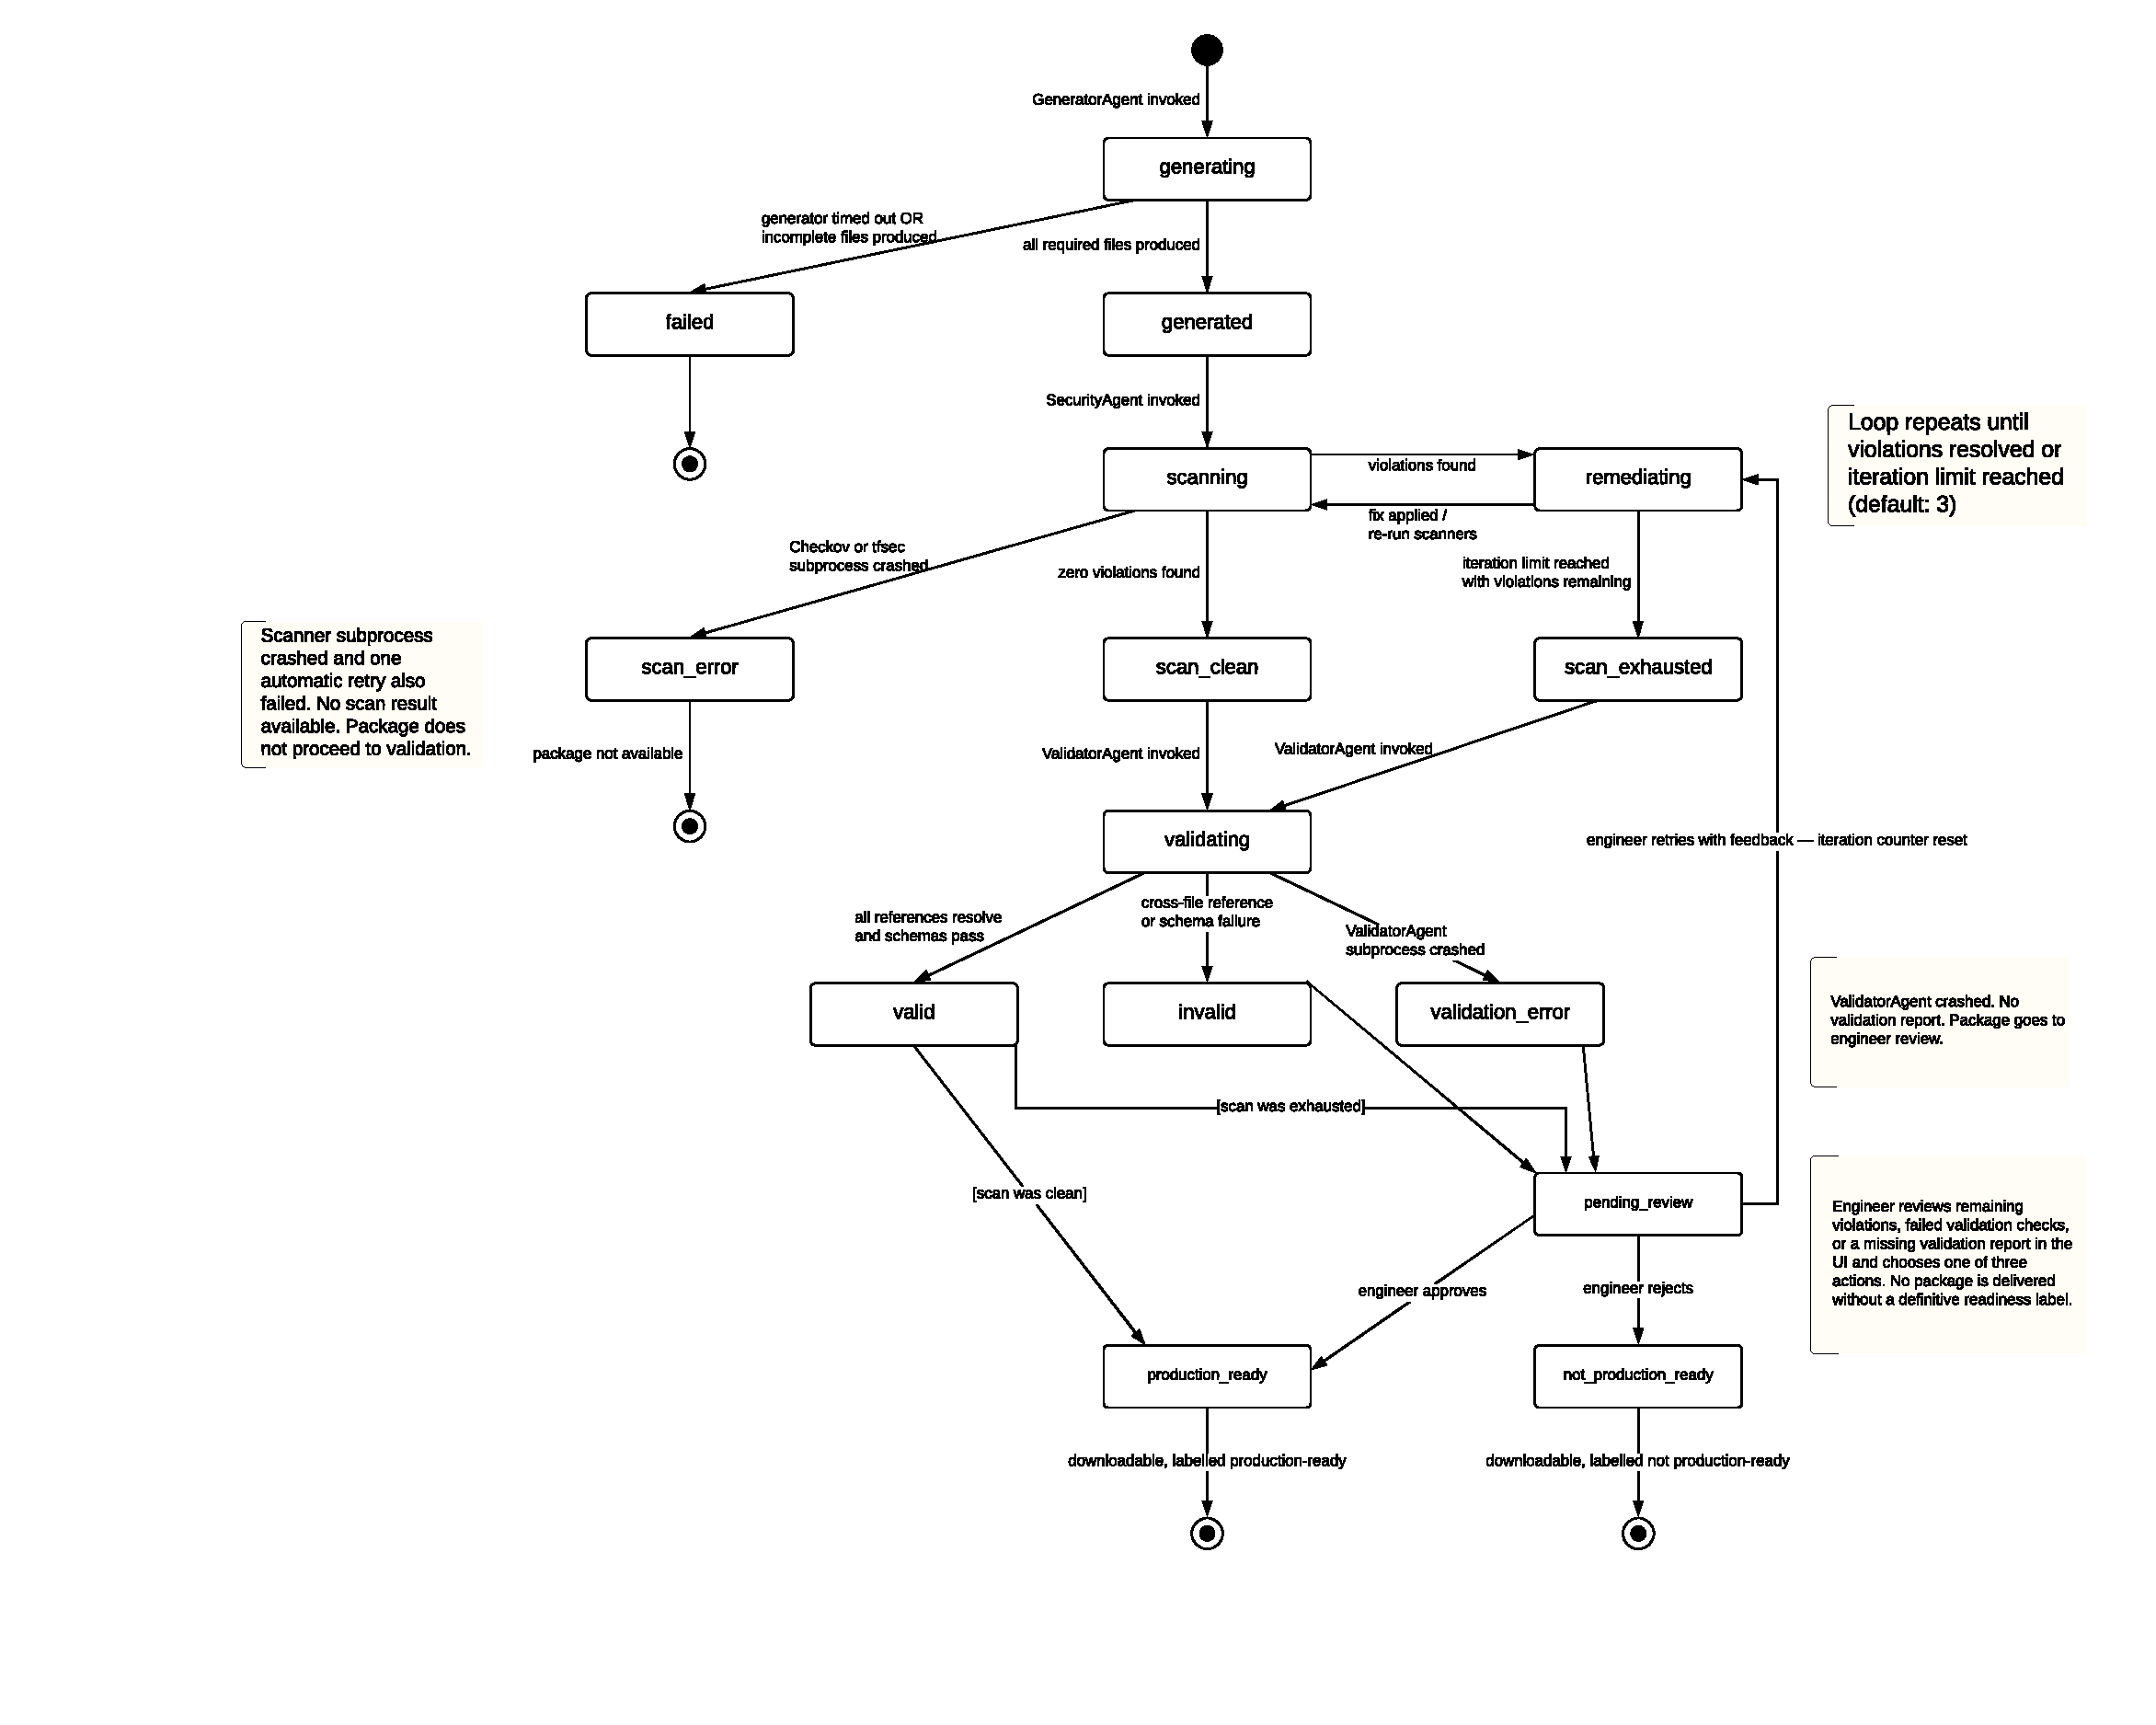
\includegraphics[width=\textwidth]{images/package_states.pdf}
  \caption{Package-level state machine. The scanning/remediating cycle on
    the left repeats until violations clear or the iteration limit is hit;
    a clean scan followed by passing validation reaches
    \texttt{production\_ready}, while an exhausted iteration budget, a
    validation failure, or a validator crash routes to
    \texttt{pending\_review}, where the engineer approves, retries with
    feedback, or rejects. Every path
    terminates at \texttt{production\_ready} or \texttt{not\_production\_ready}
    --- both downloadable, both clearly labelled. Drawn with AI-assisted
    prompting; reviewed and corrected by the author.}
  \label{fig:packagestates}
\end{figure}

Figure~\ref{fig:classdiagram} shows the class structure that encodes these
rules.

\begin{figure}[h]
  \centering
  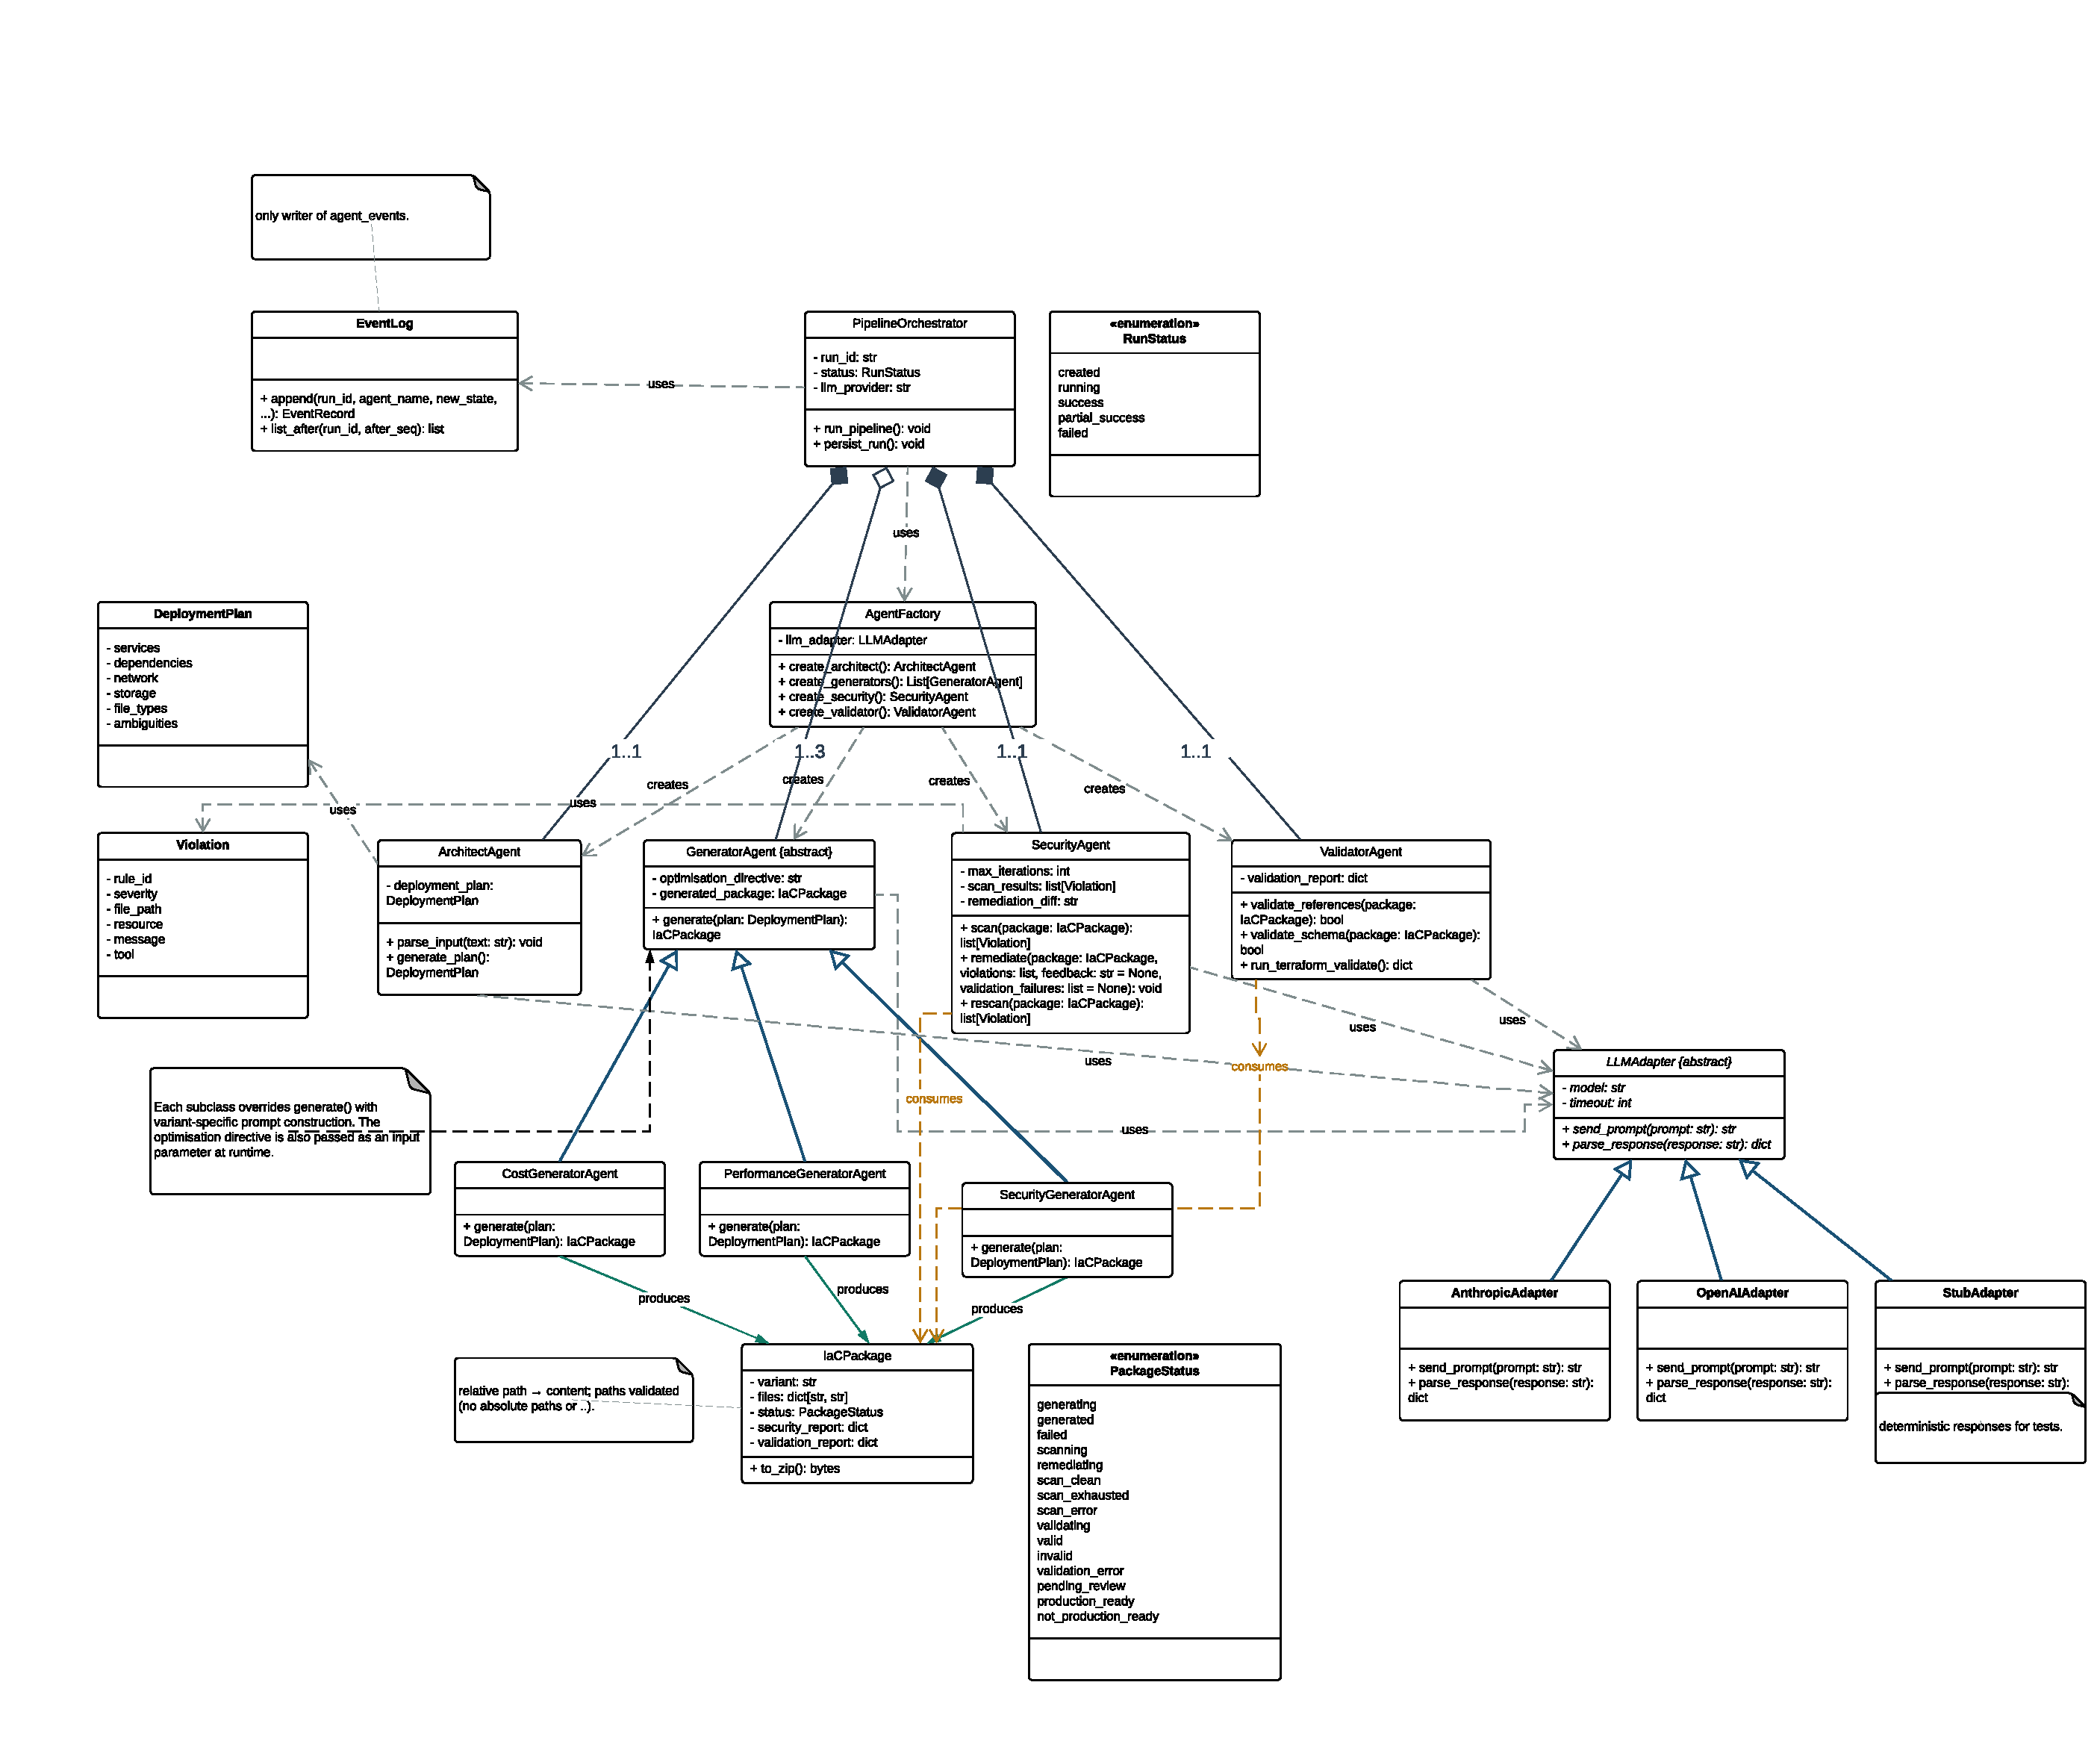
\includegraphics[width=\textwidth]{images/class_diagram.pdf}
  \caption{UML class diagram. The GeneratorAgent abstract class enforces the
    common interface; the three concrete subclasses override \texttt{generate()}
    with variant-specific prompt construction. The LLMAdapter wraps both
    supported providers behind a single two-method interface.}
  \label{fig:classdiagram}
\end{figure}

The PipelineOrchestrator composes one ArchitectAgent, one SecurityAgent, and
one ValidatorAgent (1..1 in each case) and aggregates three GeneratorAgent
instances (1..3). Composition here means the orchestrator owns those agents'
lifecycles; aggregation for the generators reflects that they run as a managed
collection rather than individually named fields.

The IaCPackage class is the data object that flows between stages. Generators
produce it; the SecurityAgent and ValidatorAgent consume it, annotating it
with scan results and validation reports as they go. Keeping it as a typed
class rather than a raw dictionary means each agent's input and output contract
is inspectable and testable in isolation.

% ---------------------------------------------------------------------------
\section{Data and Persistence Design}
\label{sec:data-design}

The system uses PostgreSQL with three tables. Figure~\ref{fig:erd} shows the
entity relationship diagram.

\begin{figure}[h]
  \centering
  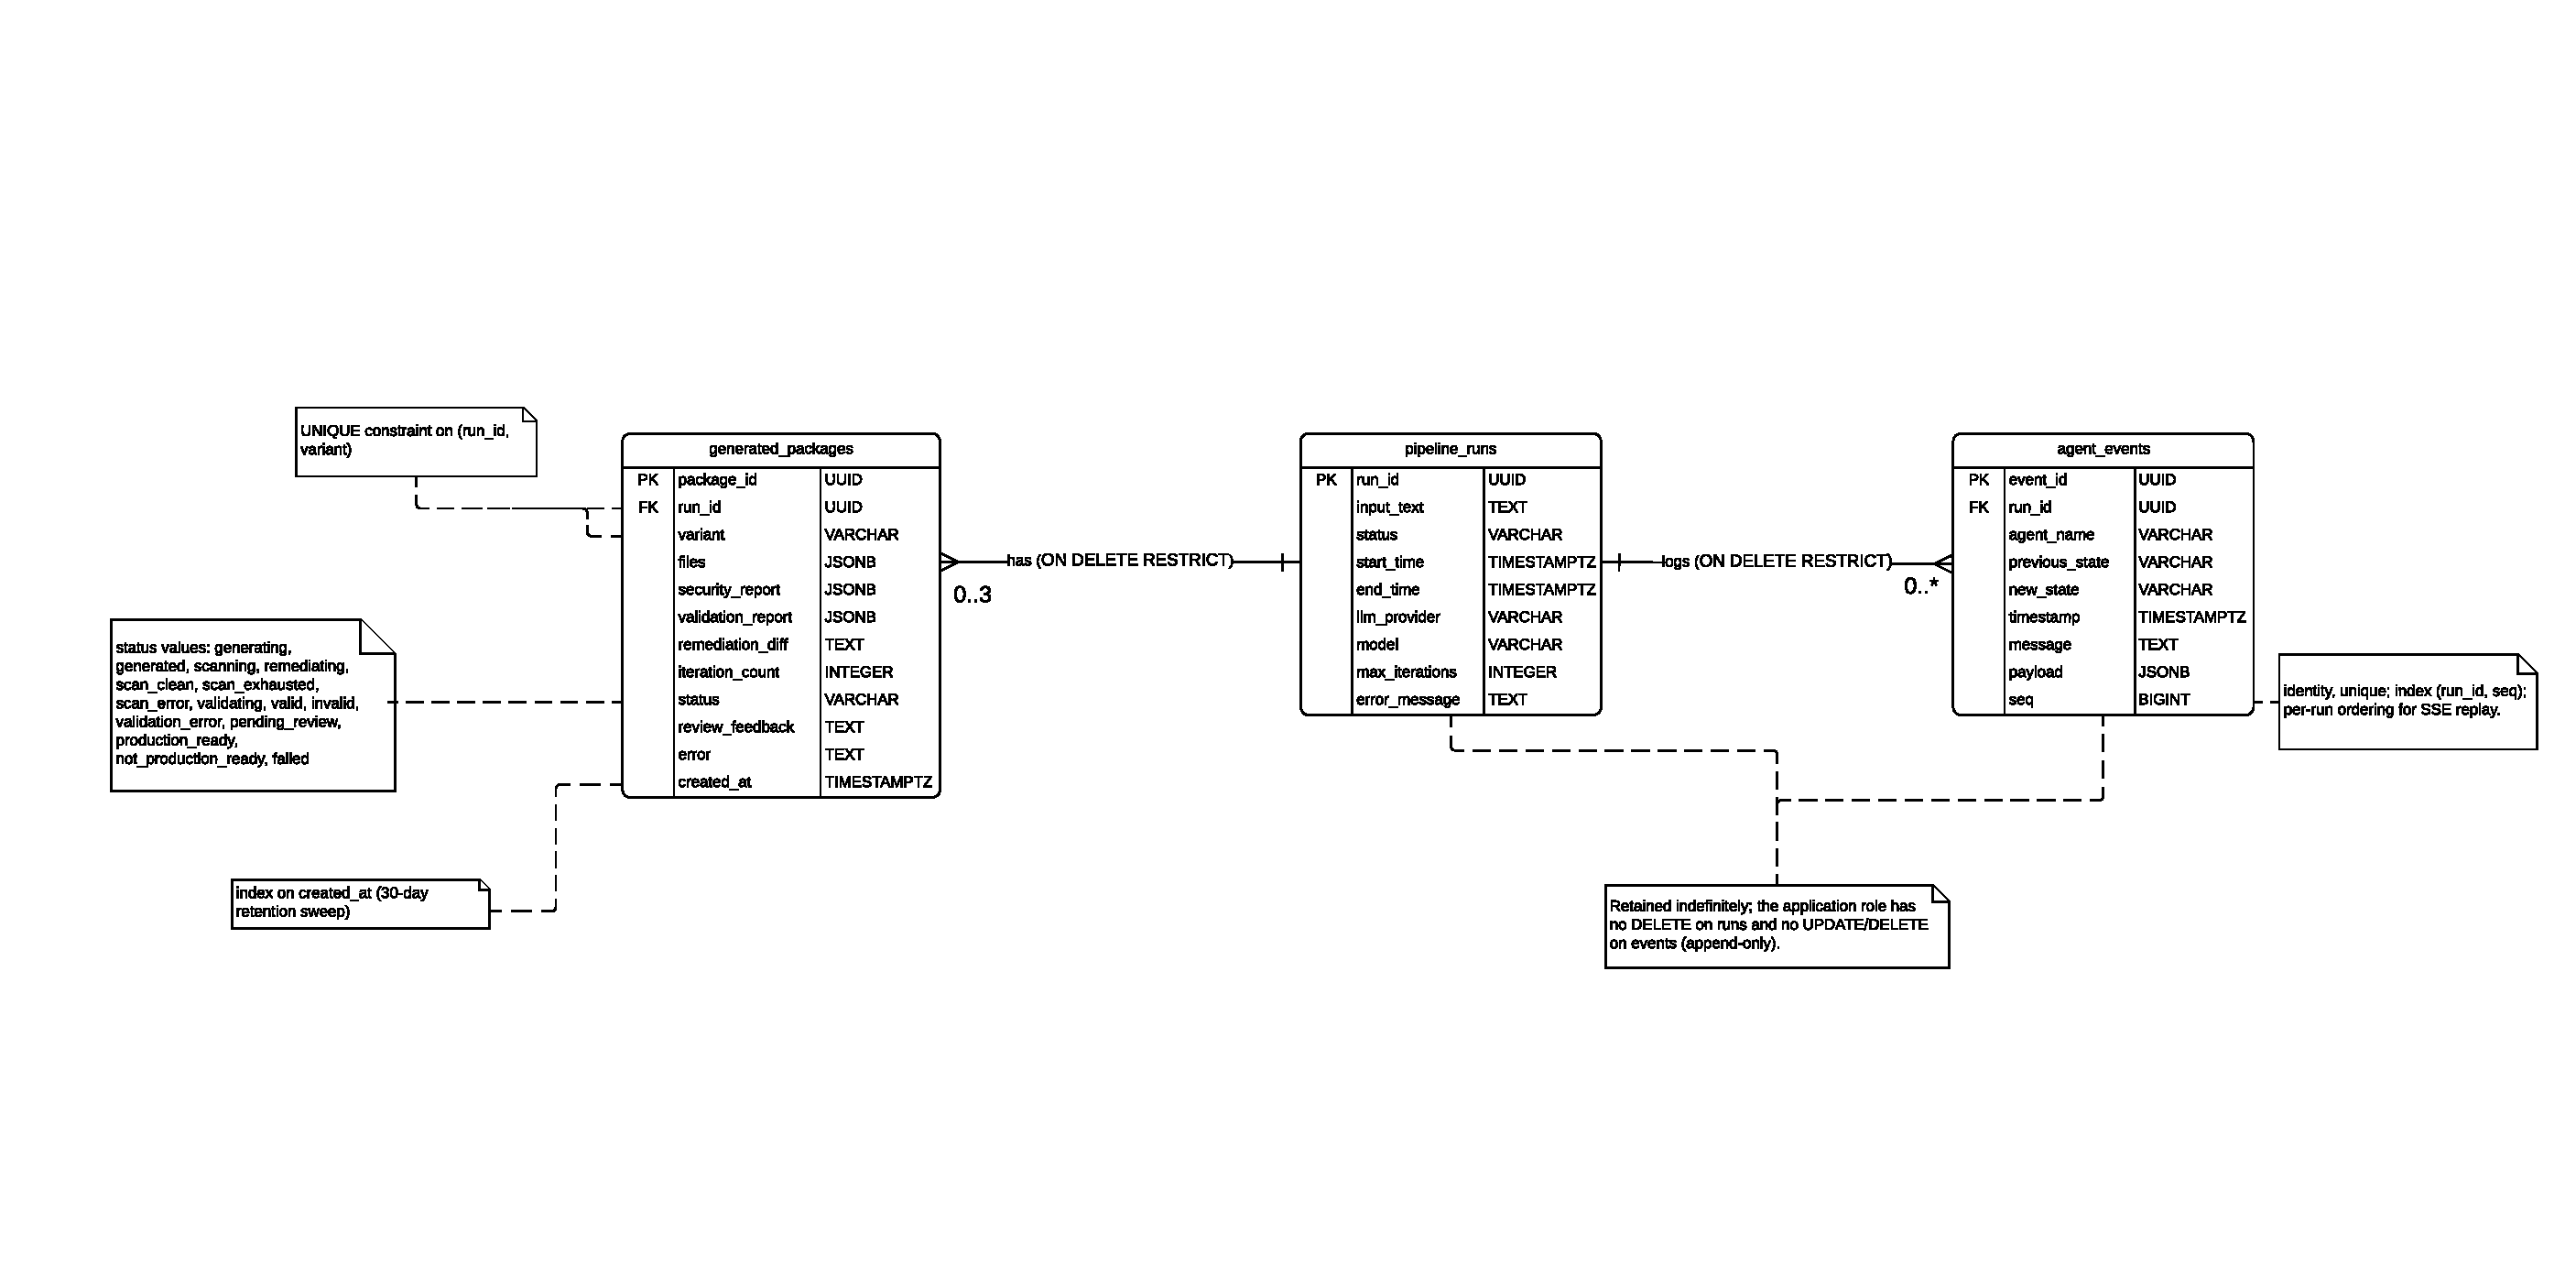
\includegraphics[width=\textwidth]{images/erd.pdf}
  \caption{Entity relationship diagram. Crow's foot notation: the single
    vertical bar on the \texttt{pipeline\_runs} side of each relationship
    denotes ``one''; the crow's foot on the child table side denotes ``many''.
    \texttt{generated\_packages.status} carries the package-level state
    machine values shown in Figure~\ref{fig:packagestates}. Drawn with
    AI-assisted prompting; reviewed and corrected by the author.}
  \label{fig:erd}
\end{figure}

\texttt{pipeline\_runs} anchors the schema. It stores one row per pipeline
execution with the input text, overall status, start and end times, LLM
provider and model, the configured maximum remediation iterations, and an
error message field for failed runs. Every other table foreign-keys back to
this one via \texttt{run\_id}.

\texttt{generated\_packages} stores one row per variant per run, with a
UNIQUE constraint on \texttt{(run\_id, variant)} so each variant appears at
most once per run. The file contents go into a JSONB column: the files are a
variable-length key-value map from filename to content string, and JSONB
handles that without requiring a fixed schema or a separate files table. The
SecurityAgent's unified diff and the ValidatorAgent's report go into their
own columns on the same row, so a single join retrieves everything the
comparison panel needs. Cardinality is 0..3 per run, reflecting that one,
two, or all three generators may succeed. The \texttt{status} column stores
the current package-level state from Figure~\ref{fig:packagestates} ---
everything from \texttt{generating} through \texttt{production\_ready} or
\texttt{not\_production\_ready} lives here as a single field, which is what
lets the API answer ``is this package still waiting on me'' with one row
read. \texttt{review\_feedback} holds whatever guidance the engineer typed
at the retry step; \texttt{error} captures scanner or validator crash
details; \texttt{created\_at} is what the 30-day retention sweep filters on.

\texttt{agent\_events} stores one row per agent state transition (0..* per
run), each carrying the \texttt{run\_id} it belongs to and a
\texttt{payload} JSONB column holding whatever structured data the event
needs --- a scan result summary, a validation report excerpt, a rejection
reason. This table drives two things simultaneously: the SSE broker at
runtime (the orchestrator writes an event, the SSE endpoint reads the
history and then subscribes to new ones) and the audit log after the fact
(a failed run's full transition history is queryable by run ID).
Separating events from run state means the orchestrator can emit a status
update without touching the \texttt{pipeline\_runs} row, which reduces
write contention on the primary table.

The schema is in third normal form. UUIDs serve as primary keys throughout
rather than auto-increment integers because the pipeline assigns a run ID
before the first database write; the ID is available immediately for the SSE
stream and the API response without a round-trip to retrieve a generated
value.

Generated package data older than 30 days is eligible for deletion.
\texttt{pipeline\_runs} and \texttt{agent\_events} rows are retained
indefinitely for audit purposes.

% ---------------------------------------------------------------------------
\section{Interfaces, API, and Interaction Design}
\label{sec:api-design}
\label{sec:sequence-design}
\label{sec:concurrency-design}

The backend exposes four REST endpoints and one SSE stream. All requests and
responses use JSON; all endpoints return standard HTTP status codes.

\begin{description}[leftmargin=3cm, style=nextline]
  \item[\texttt{POST /api/pipeline/run}]
    Accepts the natural-language input string and an optional configuration
    object. Returns a run ID immediately and begins the pipeline
    asynchronously. HTTP 422 if the input fails the infrastructure-intent
    check; HTTP 400 if the request body is malformed.

  \item[\texttt{GET /api/pipeline/\{run\_id\}/stream}]
    SSE endpoint. Every agent event is written to \texttt{agent\_events}
    first, then published to an in-memory per-run broker that this
    endpoint subscribes to. A client connecting late replays the event
    history from the database before switching to the live broker feed,
    so no state change is missed regardless of when the browser connects.
    Each event carries \texttt{agent}, \texttt{status}, and
    \texttt{message} fields. The stream stays open, or can be reopened,
    while any package in the run is in \texttt{scanning},
    \texttt{remediating}, or \texttt{validating}; this matters
    specifically for the retry path, where a package can re-enter
    remediation well after the run itself has settled into
    \texttt{partial\_success} (a run with a package awaiting review can't
    be \texttt{success}). The run's own status
    is frozen once set --- it records what the automated pipeline
    achieved, not what happens afterward at the package level. The
    connection closes once no package in the run is actively being
    worked on.

  \item[\texttt{GET /api/pipeline/\{run\_id\}/results}]
    Returns all available generated packages with their security reports and
    validation reports as a single JSON response. Called once the
    engineer sees the pipeline-complete or partial-success badge in the
    progress view.

  \item[\texttt{POST /api/pipeline/\{run\_id\}/packages/\{variant\}/review}]
    Accepts the engineer's decision on a package in
    \texttt{pending\_review}. Body: \texttt{\{action:
    "approve"|"retry"|"reject", feedback?: string\}}.
    \texttt{approve} and \texttt{reject} transition the package directly
    to \texttt{production\_ready} or \texttt{not\_production\_ready} and
    return HTTP 200. \texttt{retry} resets the iteration counter to the
    full configured limit, resumes the SecurityAgent with the optional
    feedback text and any failed checks from the validation report
    included in its next fix-generation prompt (FR-S-08
    through FR-S-10), and returns HTTP 202 since remediation continues
    asynchronously; the frontend reconnects to the SSE stream on
    receiving this response. HTTP 409 if the package isn't currently in
    \texttt{pending\_review}.

  \item[\texttt{GET /api/pipeline/\{run\_id\}/download/\{variant\}}]
    Returns a ZIP archive of the selected variant's candidate IaC files.
    Variant is one of \texttt{cost}, \texttt{performance}, or
    \texttt{security}. HTTP 404 if the variant failed to generate;
    HTTP 409 if the package is still in \texttt{pending\_review} ---
    it becomes downloadable only once the engineer resolves it via the
    review endpoint (FR-UI-06).
\end{description}

Figure~\ref{fig:sequence} shows the full pipeline interaction sequence from
input submission to file download.

\begin{figure}[h]
  \centering
  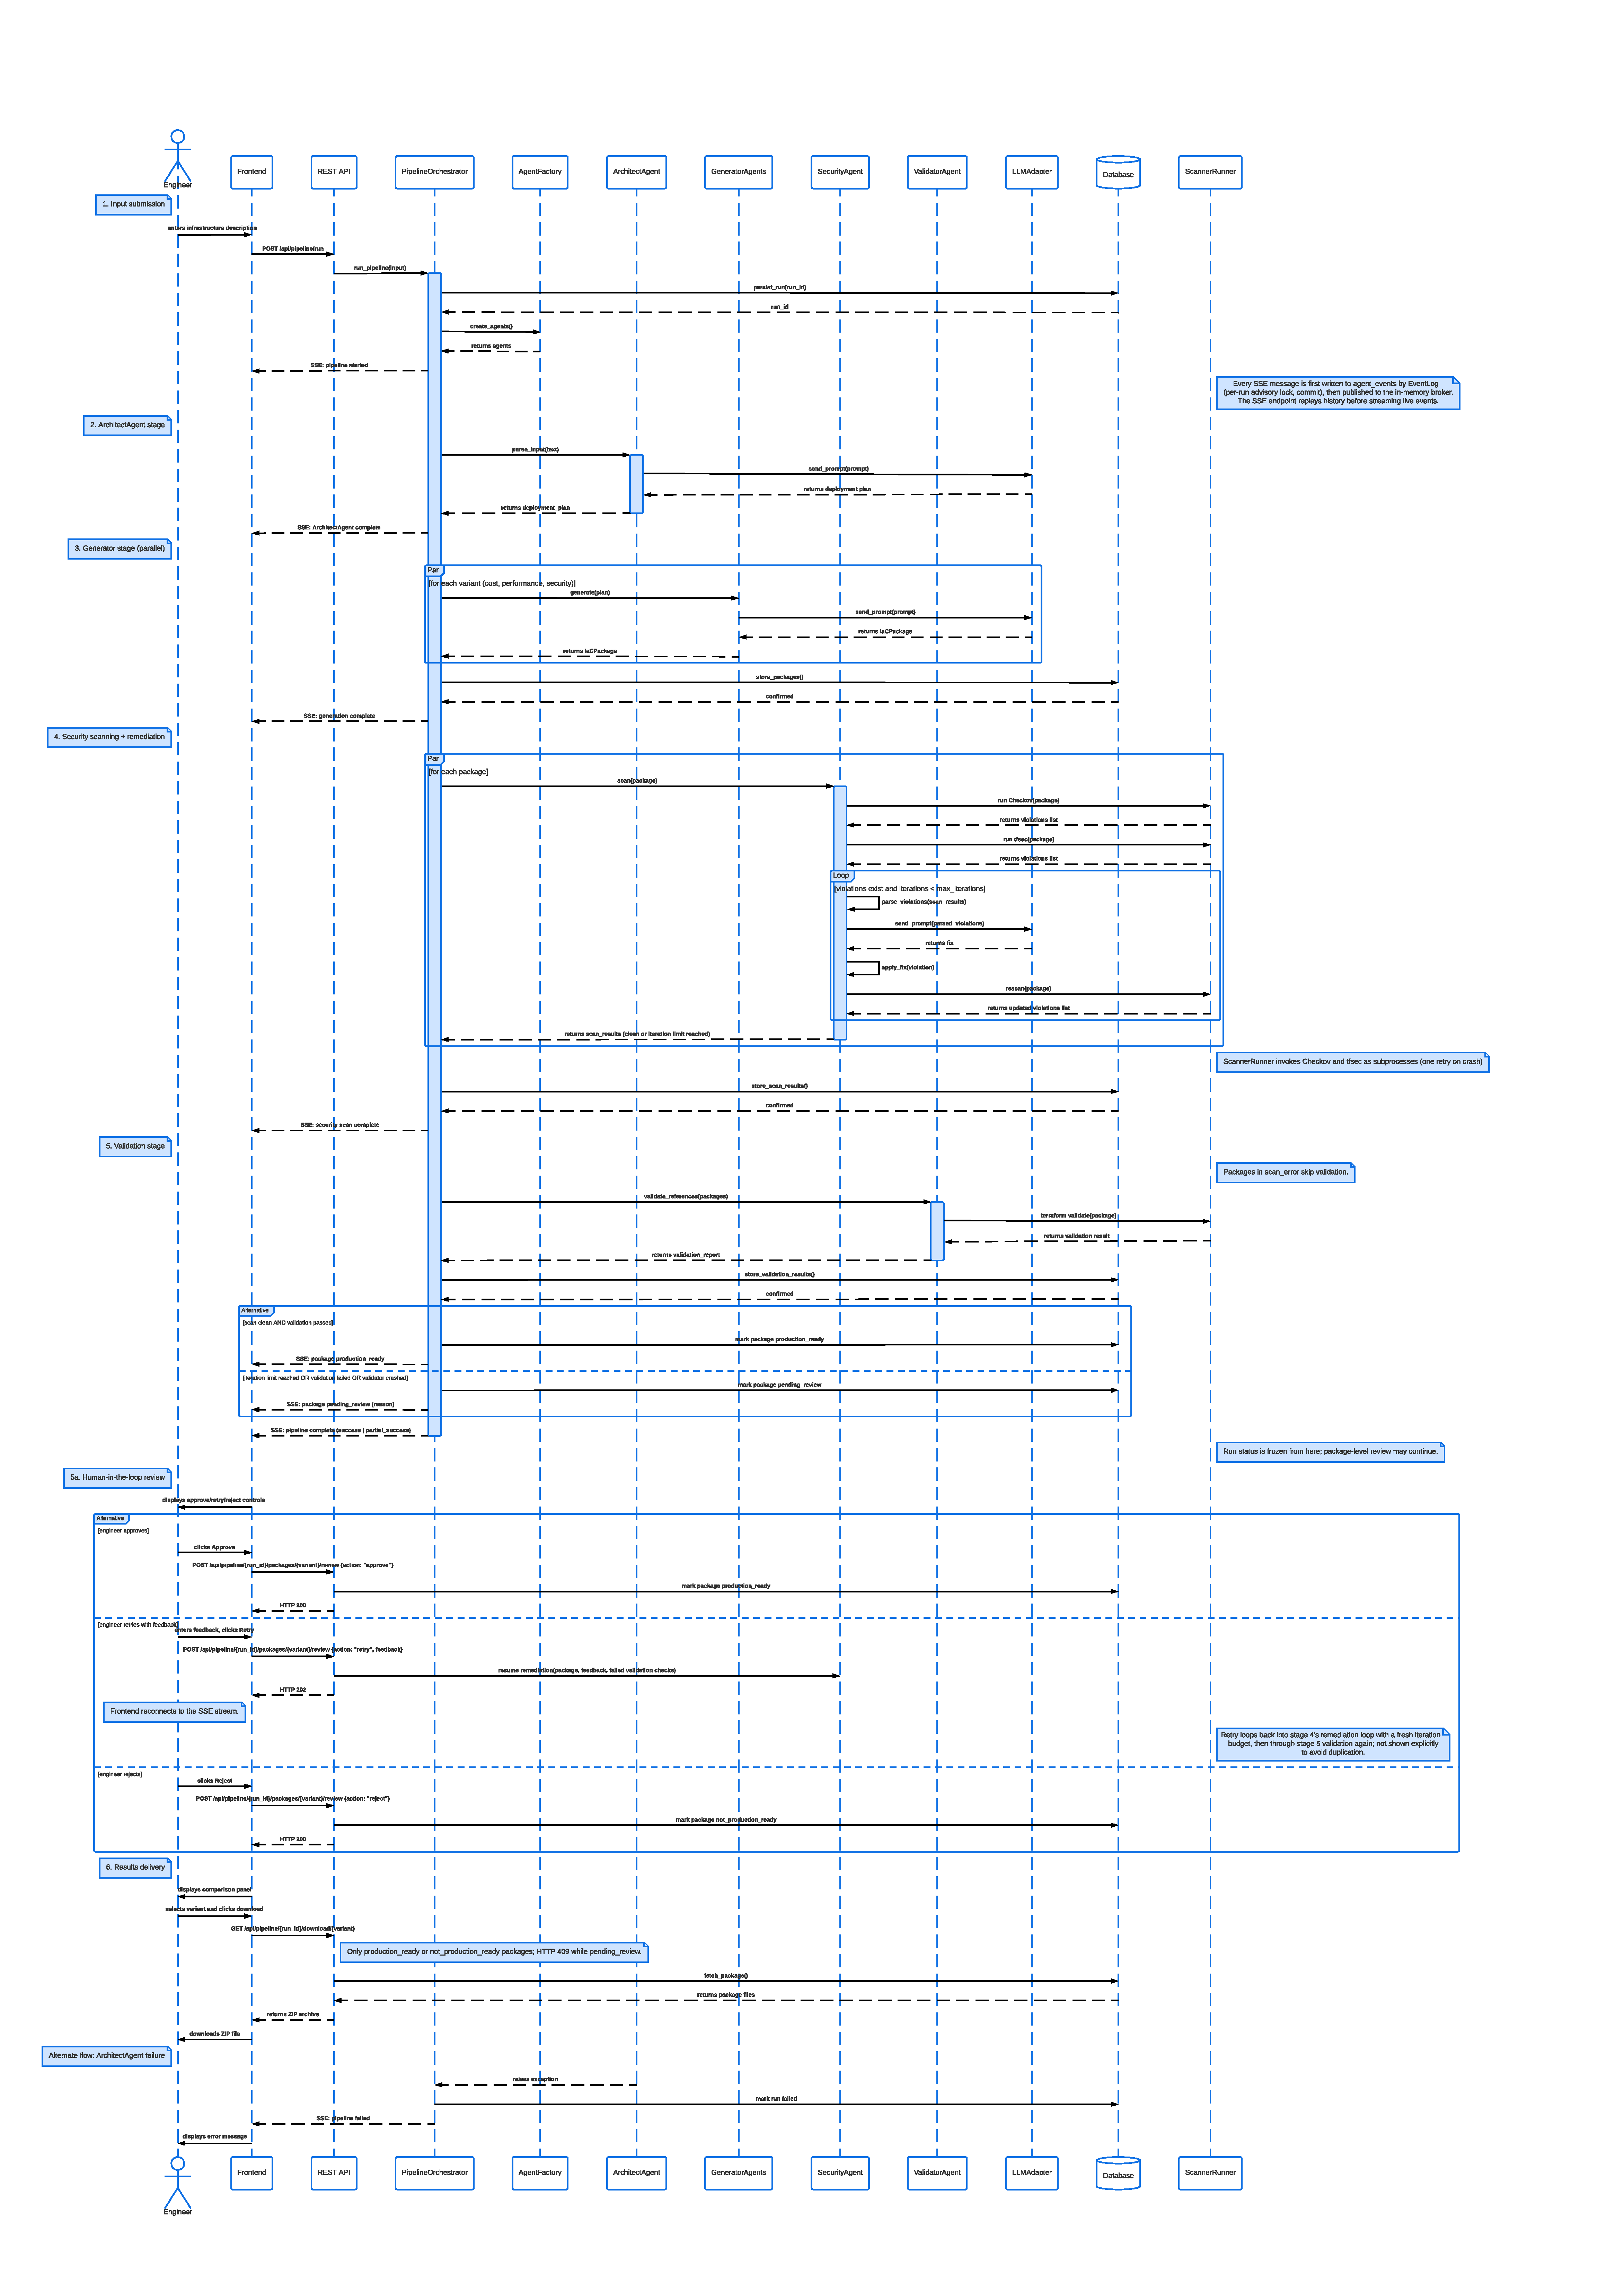
\includegraphics[width=\textwidth]{images/sequence_diagram.pdf}
  \caption{UML sequence diagram covering the full pipeline from input
    submission to file download. The dashed SSE arrows show events pushed
    from the backend to the frontend without polling. The loop fragment in
    Section 4 shows the SecurityAgent's scan-remediate-rescan cycle with
    its guard condition. Section 4a shows the human-in-the-loop review that
    follows whenever the loop exits with violations still unresolved: an
    \texttt{alt} fragment covering the engineer's three choices --- approve,
    retry with feedback, or reject.}
  \label{fig:sequence}
\end{figure}

The interaction has one non-obvious sequencing constraint: the orchestrator
persists the run ID to PostgreSQL before invoking the ArchitectAgent. If the
ArchitectAgent call fails on the first attempt, the run record already exists
and the engineer can retrieve the error by run ID without losing the input
text.

The LLM API interface enforces a 150-second total timeout per agent (30 seconds
per call attempt, up to 3 attempts with exponential backoff, maximum 150 seconds
total including backoff delays) before the pipeline marks the agent as failed
(FR-A-04). Plain-text responses from the LLM are treated
as errors; agents only accept structured JSON. This constraint comes from
operational experience: LLMs occasionally return explanatory prose when they
can't satisfy a prompt, and silently treating that as valid JSON produces
incorrect IaC files rather than a visible failure.

% ---------------------------------------------------------------------------
\section{User-Interface and Accessibility Design}
\label{sec:ui-design}

The interface follows a linear four-screen flow. The visual theme uses dark
navy backgrounds, orange accents, and monospace fonts for code and log output,
matching the AWS Console aesthetic that DevOps engineers already work in daily.

\textbf{Screen 1 -- Input view} (Figure~\ref{fig:screen1}). A single text
area with placeholder guidance, a character counter, a collapsible
configuration panel for LLM provider and iteration settings, and an orange
generate button. Three example prompt chips let engineers populate the text
area with one click for common deployment patterns. The submit button disables
on submission and re-enables only when the pipeline reaches a terminal state
(FR-UI-01).

\begin{figure}[h]
  \centering
  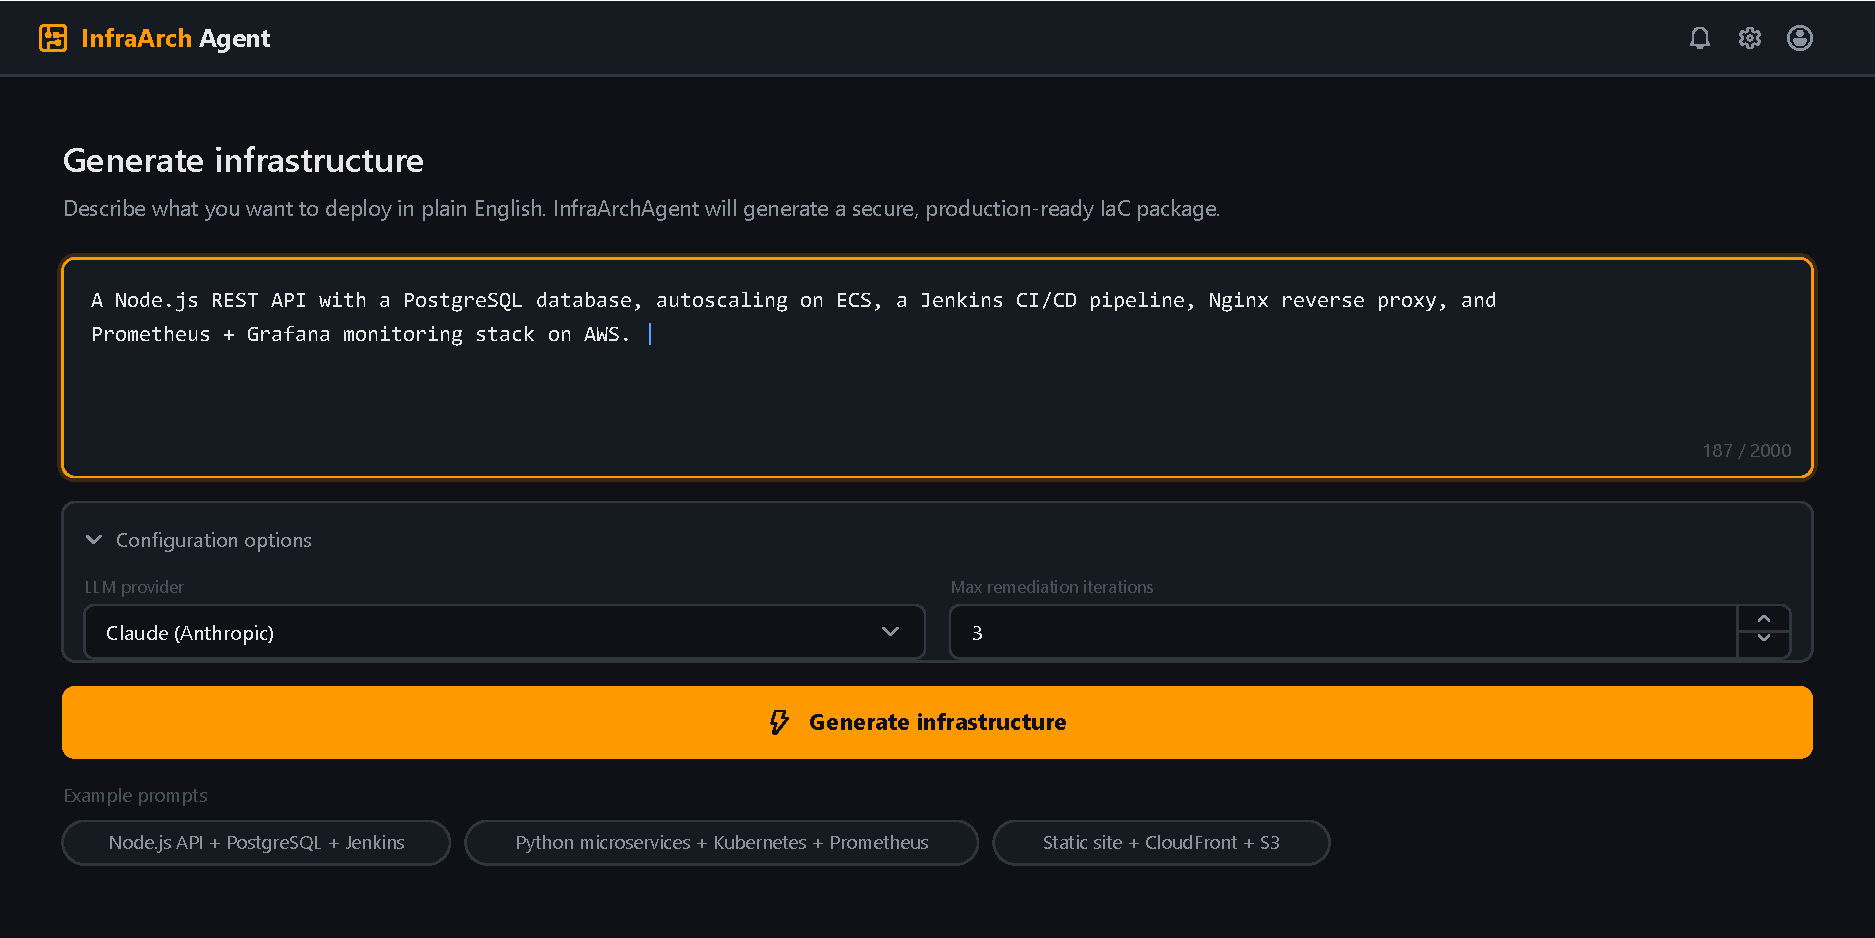
\includegraphics[width=\textwidth]{images/screen1_input.pdf}
  \caption{Input view. The configuration panel is collapsed by default;
    engineers who accept the defaults never need to open it.}
  \label{fig:screen1}
\end{figure}

\textbf{Screen 2 -- Pipeline progress} (Figure~\ref{fig:screen2}). Four
stage cards update in real time via the SSE stream, each showing agent name,
status badge (green for complete, blue for running, gray for queued), elapsed
time, and a one-line log message. The GeneratorAgents card expands to show
per-variant sub-status. A scrolling log panel below shows the raw event stream
in monospace text. The entire view updates without page refresh (FR-UI-02).

\begin{figure}[h]
  \centering
  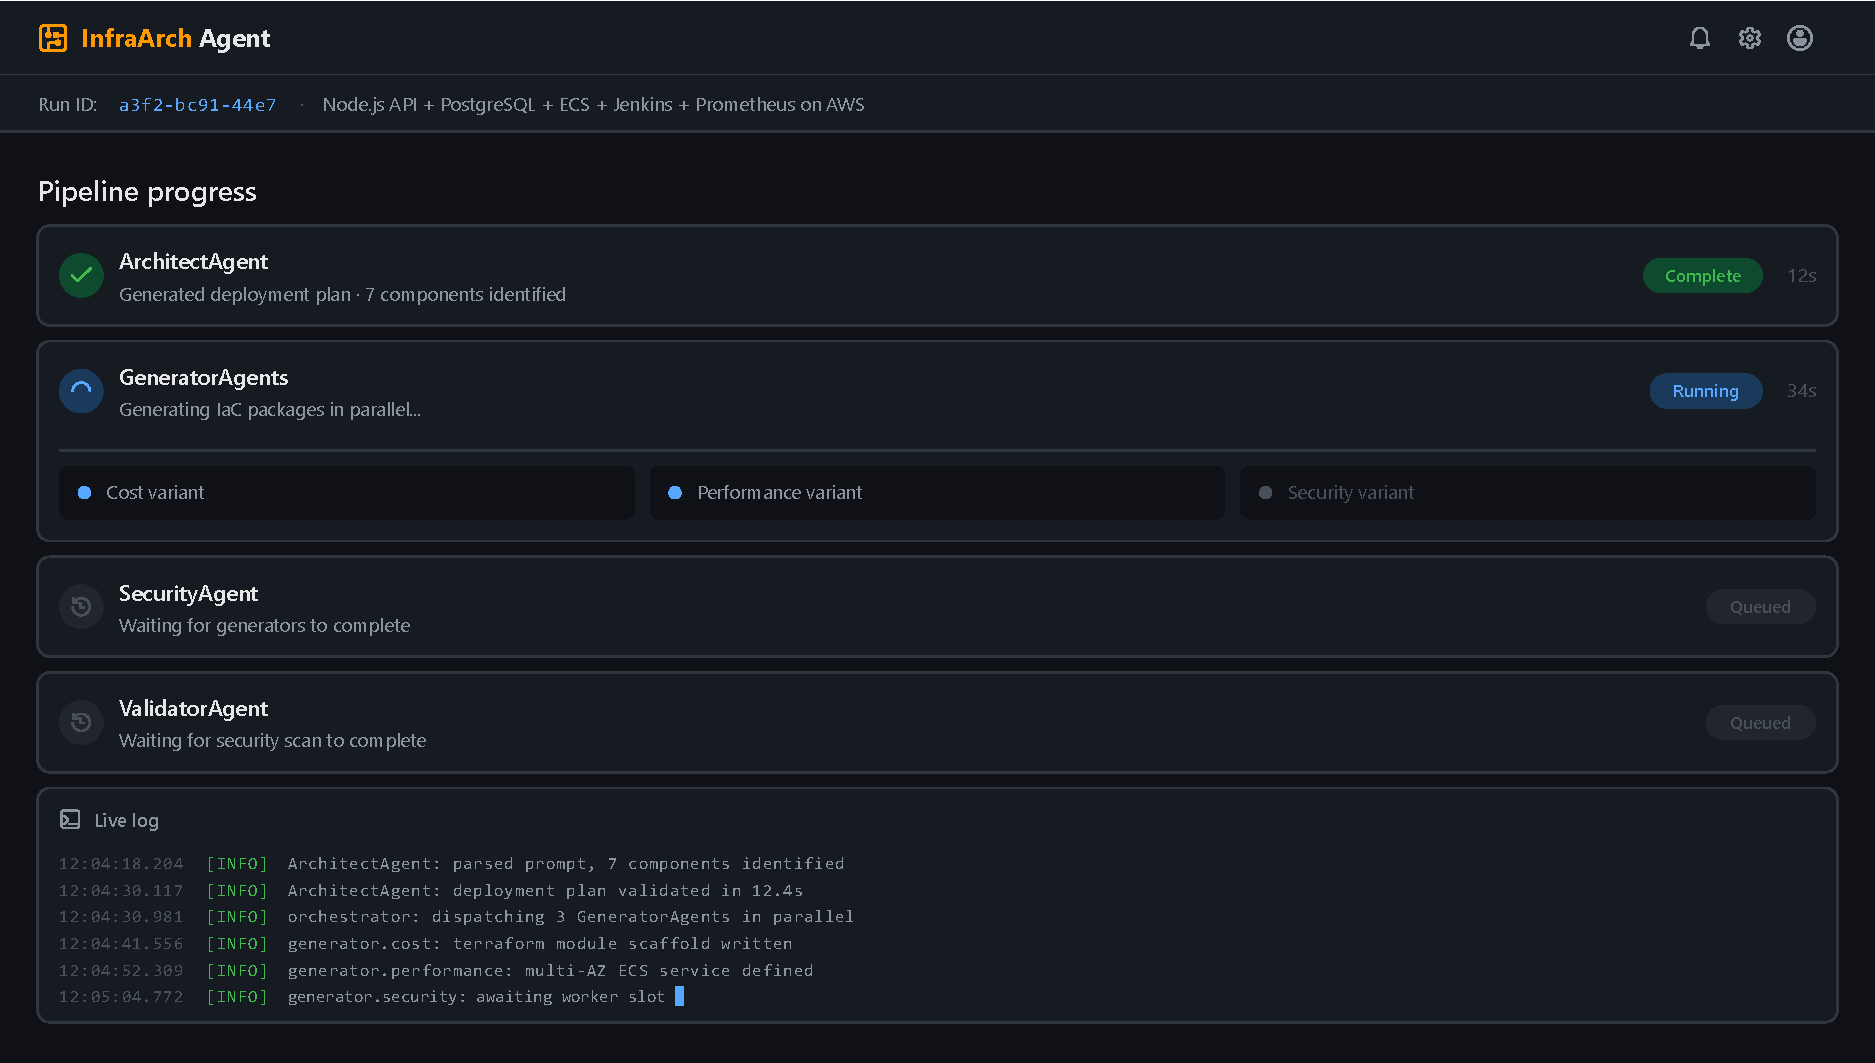
\includegraphics[width=\textwidth]{images/screen2_progress.pdf}
  \caption{Pipeline progress view mid-run. Two generator variants are running
    (blue); the security variant is queued (gray); the ArchitectAgent has
    already completed (green).}
  \label{fig:screen2}
\end{figure}

\textbf{Screen 3 -- Comparison panel} (Figure~\ref{fig:screen3}). Up to
three columns, one per available variant, each showing the optimisation badge,
security score, and a navigable file tree. Missing variants show a failure
note instead of a column. The selected variant gains an orange border. The
engineer picks a variant here before moving to the diff view (FR-UI-03).

\begin{figure}[h]
  \centering
  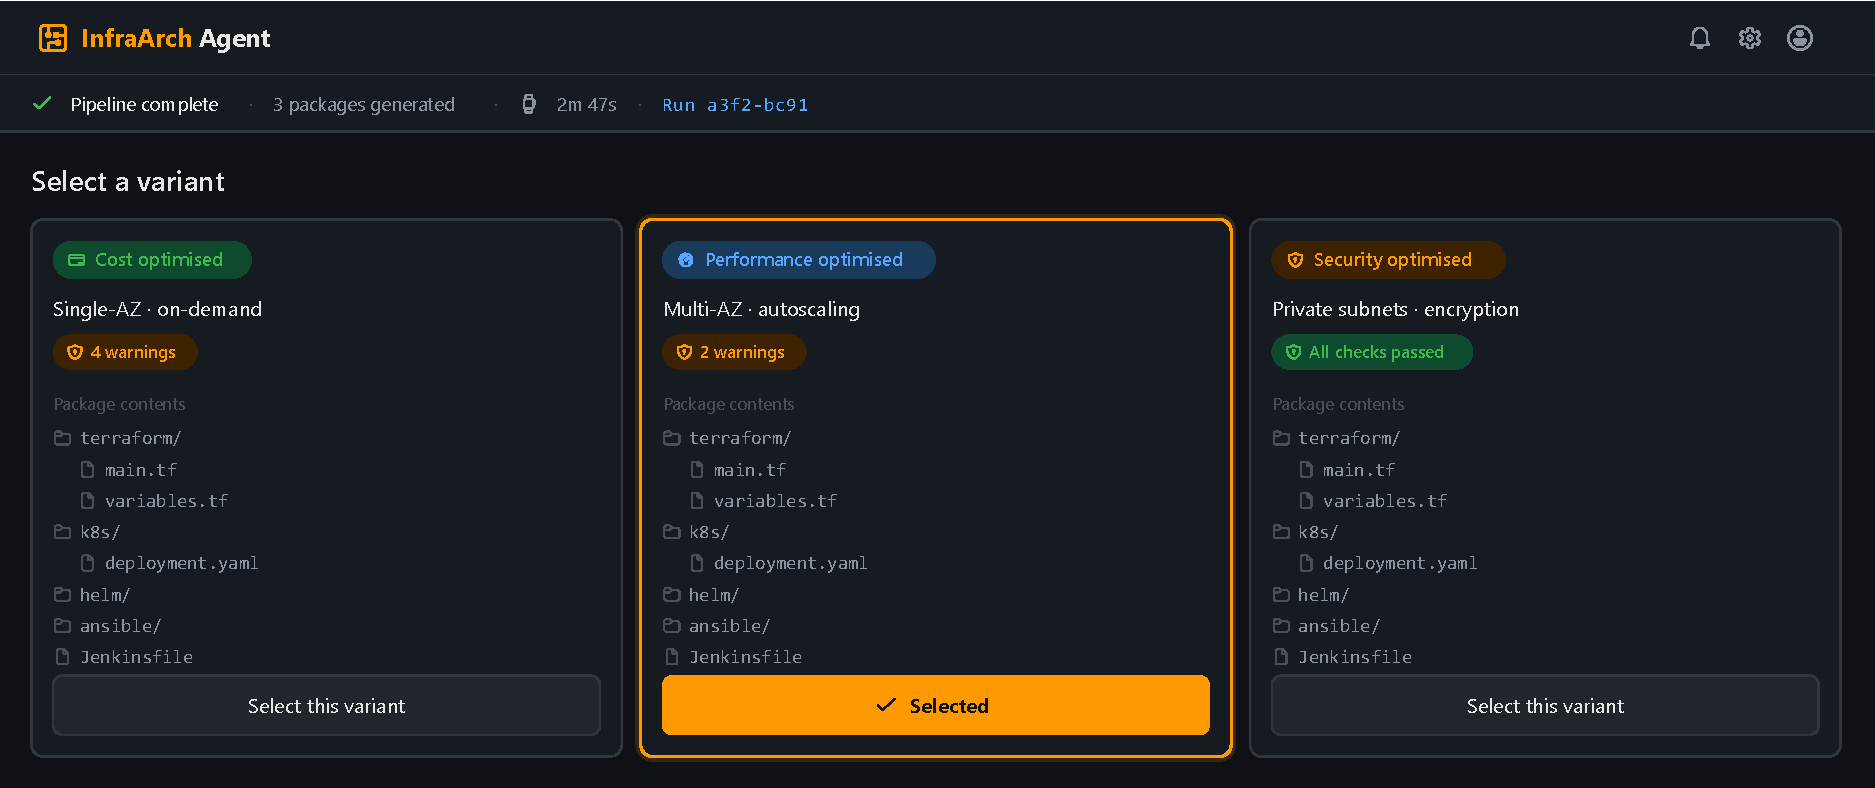
\includegraphics[width=\textwidth]{images/screen3_comparison.pdf}
  \caption{Comparison panel after a completed run. The performance-optimised
    column is selected (orange border). Security scores vary across variants
    because each generator takes a different approach to IAM and encryption.}
  \label{fig:screen3}
\end{figure}

\textbf{Screen 4 -- Diff and download} (Figure~\ref{fig:screen4}). A file
sidebar on the left, a code diff in the center (red for removed lines, green
for added lines, each annotated with the Checkov or tfsec rule that triggered
the change), and the security fix list on the right with severity badges.
Unresolved violations appear in a distinct colour from resolved ones. When a
package is in \texttt{pending\_review}, the view shows why: outstanding
violations, failed validation checks, or a warning that the ValidatorAgent
produced no report (UC-08). Three controls replace the download
button in the navigation bar: Approve, Retry with feedback (opening a text
field for the engineer's guidance), and Reject (FR-UI-07). Once the engineer
acts, the package settles into \texttt{production\_ready} or
\texttt{not\_production\_ready} and the controls give way to the ordinary
download button, which returns a ZIP archive labelled accordingly
(FR-UI-04 through FR-UI-06).

\begin{figure}[h]
  \centering
  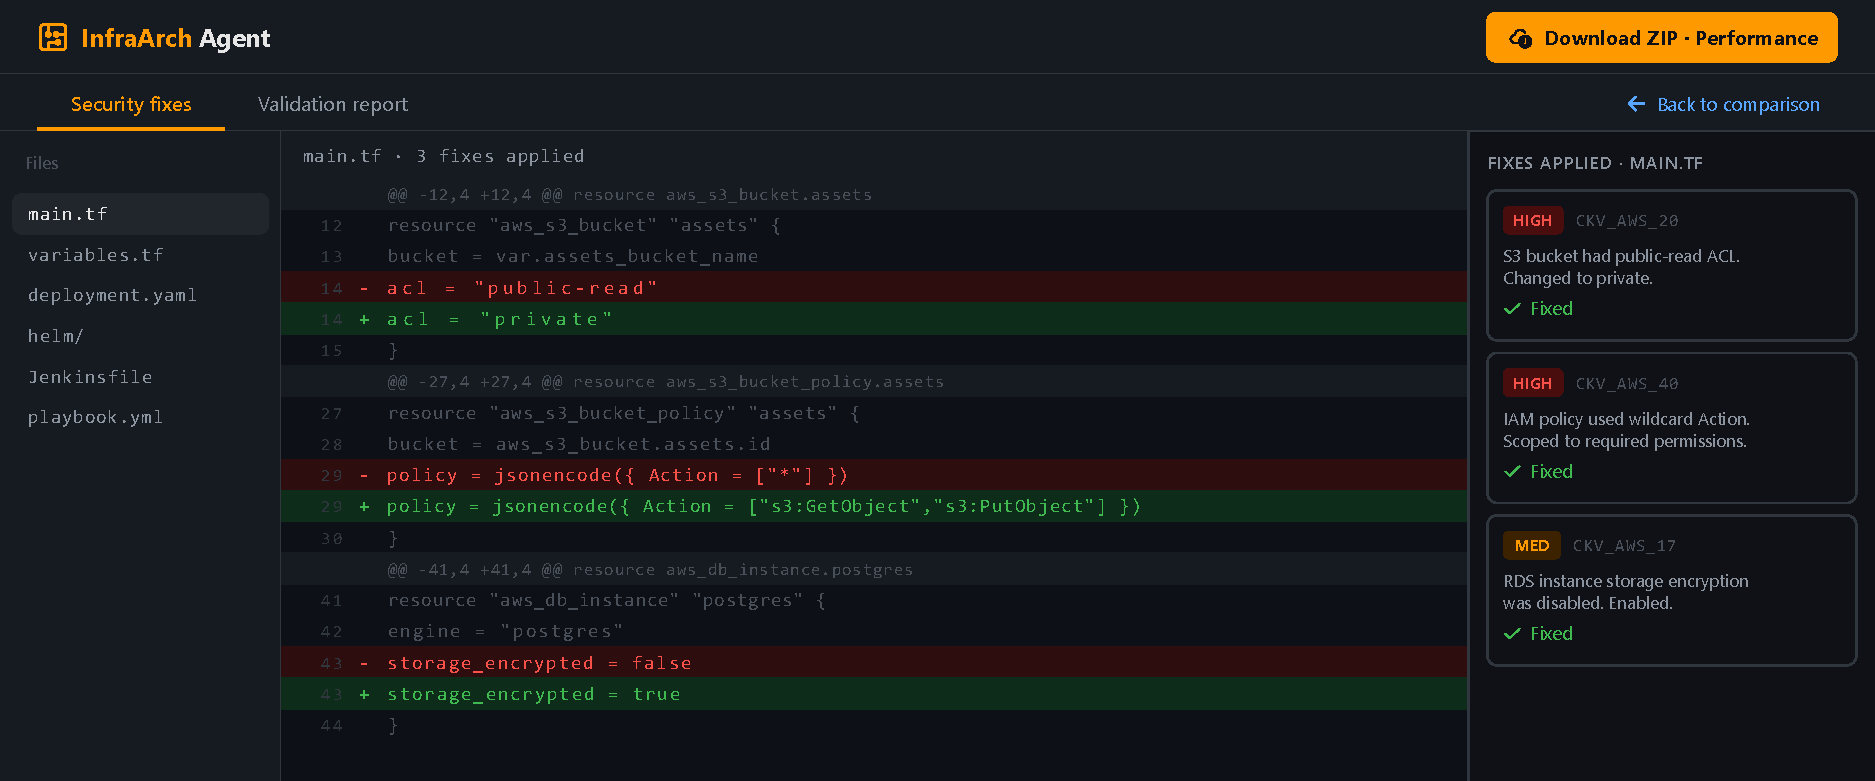
\includegraphics[width=\textwidth]{images/screen4_diff.pdf}
  \caption{Diff and download view. The center panel shows three remediated
    violations in \texttt{main.tf}: a public S3 ACL, a wildcard IAM policy,
    and disabled RDS encryption. All three are marked fixed in the right
    panel. A package still in \texttt{pending\_review} would show the
    approve/retry/reject controls here instead of the download button.}
  \label{fig:screen4}
\end{figure}

% ---------------------------------------------------------------------------
\section{Security, Privacy, and Failure Design}
\label{sec:security-design}

The system has four security-relevant assets: the LLM API key, the generated
IaC files, the pipeline run history, and the engineer's natural-language input.

The LLM API key is stored as an environment variable and never written to the
database, included in API responses, or emitted in logs (NFR-01). The backend
validates all incoming request payloads against a schema before any agent
processes them; unvalidated input never reaches the pipeline. Generated files
are stored server-side and accessed only via the download endpoint, which is protected at the server level by API key authentication rather than per-user session management; the
engineer's browser never holds the files until they explicitly request a
download.

The trust boundary sits at the REST API layer. The frontend is untrusted;
every request it sends passes through schema validation before touching the
orchestrator. The LLM API is trusted for content but not for availability;
the retry logic with exponential backoff handles transient failures, and a
three-strike timeout marks the agent as failed rather than hanging
indefinitely.

Failure modes and mitigations by component:

\begin{itemize}
  \item \textbf{LLM API timeout}: exponential backoff, three retries, then
    agent marked failed and run halted or continued depending on which agent
    timed out (FR-P-03).
  \item \textbf{Checkov or tfsec subprocess failure}: one automatic retry;
    if the retry also fails, the package enters \texttt{scan\_error}, does
    not proceed to validation, and is not available to the engineer. If
    every package ends in \texttt{scan\_error}, the run is \texttt{failed}.
  \item \textbf{ValidatorAgent crash}: the package enters
    \texttt{validation\_error}, has no validation report, and goes to
    \texttt{pending\_review} with a warning; it is never labelled
    production-ready without review.
  \item \textbf{Single generator failure}: non-fatal; the pipeline transitions
    to \texttt{partial\_success} with the remaining variants provided at least
    one completed (FR-G-06).
  \item \textbf{ArchitectAgent failure}: fatal; the pipeline halts and the
    run is marked \texttt{failed} with the error persisted for retrieval
    by run ID (FR-P-03).
  \item \textbf{Database write failure}: the pipeline surfaces an HTTP 500
    to the frontend; the SSE stream closes; the engineer sees a failure
    message and can resubmit.
  \item \textbf{Package stuck at \texttt{pending\_review}}: not treated as
    a system failure. The run itself completes normally as
    \texttt{partial\_success}, since a package in review means the run did
    not finish cleanly; the outstanding package simply waits for
    the engineer's decision. There's no timeout on this state --- rushing
    a human into a security call defeats the purpose of asking them at all.
\end{itemize}

% ---------------------------------------------------------------------------
\section{Decisions, Alternatives, and Trade-offs}
\label{sec:decisions}

\begin{longtable}{@{}p{0.16\textwidth}p{0.25\textwidth}p{0.24\textwidth}p{0.24\textwidth}@{}}
\caption{Architectural decision summary.}\label{tab:decisions}\\
\toprule
\textbf{Decision} & \textbf{Chosen option and rationale} & \textbf{Rejected alternative} & \textbf{Consequences / evidence} \\
\midrule
\endfirsthead
\toprule
\textbf{Decision} & \textbf{Chosen option and rationale} & \textbf{Rejected alternative} & \textbf{Consequences / evidence} \\
\midrule
\endhead

ADR-01 &
  Python asyncio for parallel generation. Agents spend almost all their time
  waiting for LLM responses and subprocess output; async I/O handles that
  without thread management overhead. Satisfies FR-G-01 and PR-03. &
  Python threading. Threads add synchronisation complexity and are subject
  to the GIL for CPU-bound work; the pipeline's bottleneck is I/O, not CPU. &
  Three generators fire concurrently; benchmark target is all three completing
  within 150 seconds (PR-05). Deadlock risk is absent because generators share
  no mutable state. \\

ADR-02 &
  Model-agnostic LLM adapter wrapping Anthropic and OpenAI behind
  \texttt{send\_prompt} / \texttt{parse\_response}. Satisfies NFR-03 and
  FR-I-04. &
  Hard-coding Claude or GPT-4o directly inside each agent. Would couple every
  agent to a specific SDK and make provider switching a cross-codebase change. &
  Adding a third provider requires one new adapter class. Tested by the
  stub-provider integration test in TC-adapter-01. \\

ADR-03 &
  PostgreSQL with JSONB for generated file contents. Allows variable-length
  key-value file maps without a fixed schema, and supports indexing and
  querying by filename without a separate files table. &
  Storing files on disk with paths in the database. Disk storage complicates
  cleanup, backup, and concurrent access; JSONB keeps everything in one
  transactional system. &
  Package data older than 30 days is eligible for deletion via a simple
  \texttt{DELETE WHERE created\_at < now() - interval '30 days'}. \\

ADR-04 &
  SSE for real-time pipeline progress updates. One-directional server-push
  over HTTP; no WebSocket handshake overhead; trivially supported by FastAPI
  and all modern browsers without plugins. Satisfies FR-P-04 and PR-02. &
  WebSockets. Bidirectional communication is unnecessary here; the browser
  never needs to send data after the initial POST. WebSockets add connection
  management complexity for no benefit in this use case. &
  Each agent state transition emits one SSE event; the frontend updates within
  1 second (PR-02). Verified by the SSE integration test in TC-pipeline-01. \\

ADR-05 &
  AWS as the sole target cloud provider. Checkov and tfsec have their most
  mature rulesets for AWS; the LLM has the most training data on AWS resource
  types; limiting scope makes security scanning reliable and testable. &
  Cloud-agnostic generation supporting AWS, Azure, and GCP simultaneously.
  Would require three separate generator prompt sets, three scanner
  configurations, and triples the test surface for an initial release. &
  The architecture supports extension; GeneratorAgents accept a
  \texttt{cloud\_provider} directive alongside the optimisation directive,
  so adding Azure support means new prompt templates, not new classes. \\

ADR-06 &
  Strategy pattern for the three GeneratorAgents. All three share the
  \texttt{generate(plan: dict) -> IaCPackage} interface; the optimisation
  directive is passed as an input parameter at runtime alongside the plan.
  The three concrete subclasses each override \texttt{generate()} with
  variant-specific prompt construction. Both the subclass distinction and
  the runtime directive are present and complementary. &
  Three entirely separate agent classes with no shared interface. Would
  duplicate the LLM call logic and make adding a fourth variant a copy-paste
  operation rather than a new subclass. &
  New variants require subclassing GeneratorAgent and overriding one method.
  The orchestrator needs no changes. \\

\bottomrule
\end{longtable}